\section{Method}
\label{sec:method}

\subsection{Environments and episodes}
\label{sec:envs}

\begin{figure}[t]
  \centering
  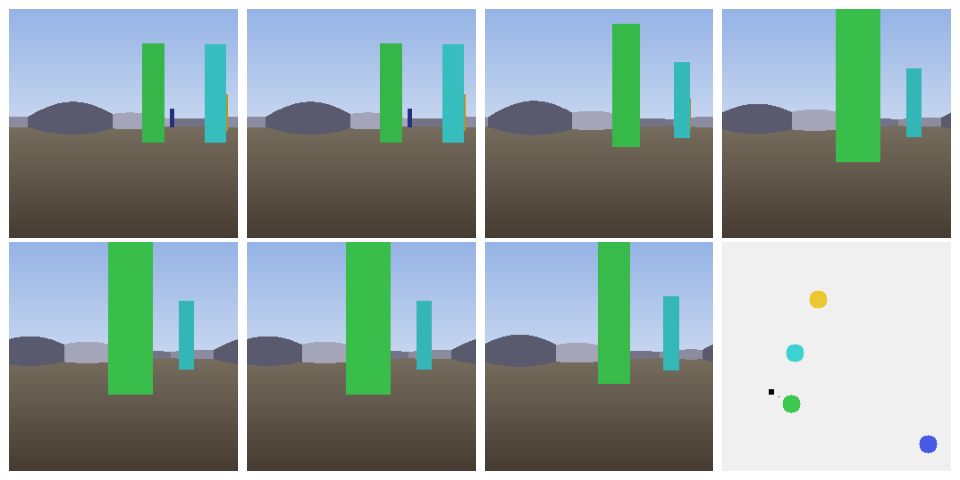
\includegraphics[width=0.49\linewidth]{fig/env_nav.png}\hfill
  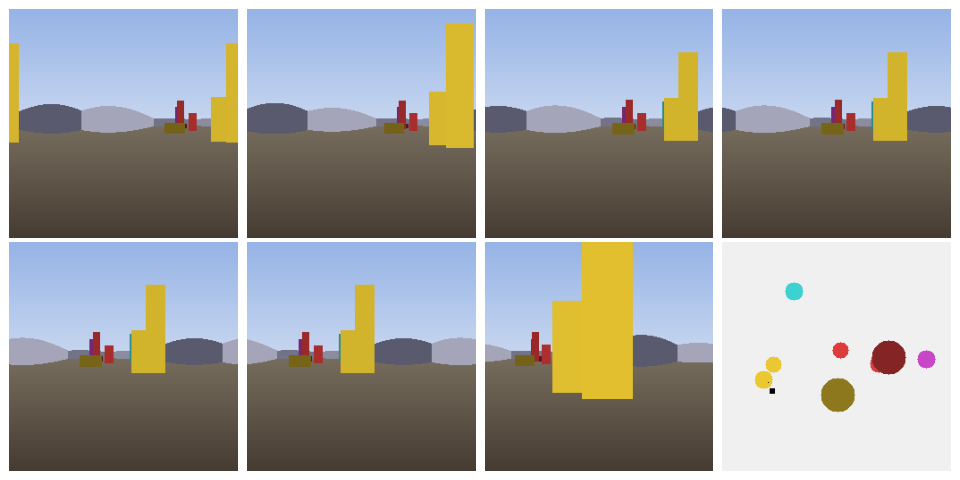
\includegraphics[width=0.49\linewidth]{fig/env_arrange.png}\\[2pt]
  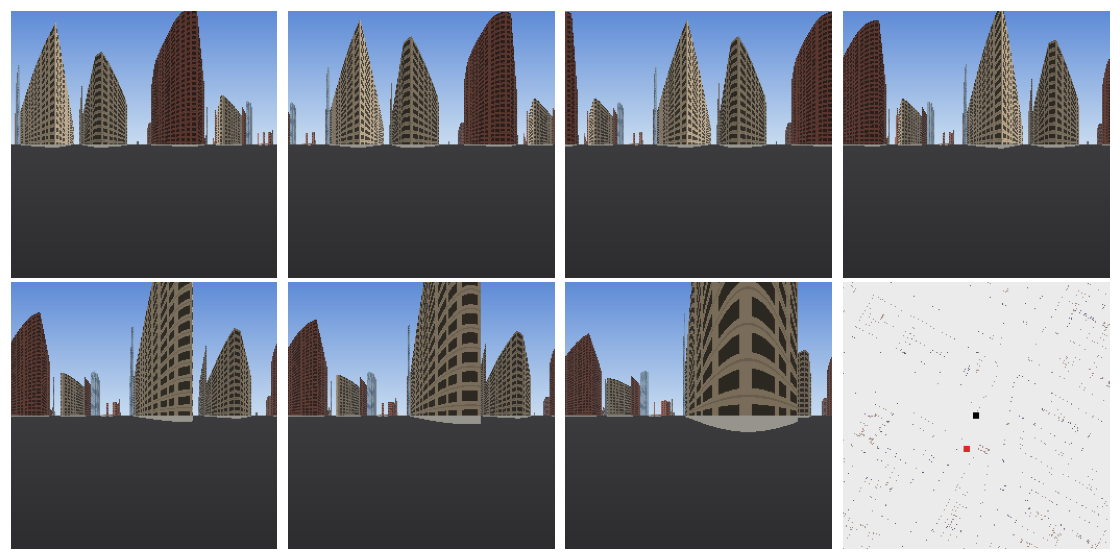
\includegraphics[width=\linewidth]{fig/env_nyc.png}
  \caption{\textbf{Environments.} Top: the 360\degree\ arena as the teacher sees it, for the \textsc{nav} (left) and
  \textsc{arrange} (right) tasks. Bottom: seven steps of one episode in the raycast twin of Midtown Manhattan and its
  top-down map (start in black, goal in red).}
  \label{fig:envs}
\end{figure}

\paragraph{Arena} A 360\degree\ cylindrical panorama rendered at 256\,px with coloured blocks on a ground plane
(\cref{fig:envs}, top). Two tasks share the action space: \textsc{nav} (reach a target block) and \textsc{arrange}
(push blocks to a layout). Five discrete actions: stay, forward 0.6 units, turn left or right 22.5\degree, back 0.36.
Episodes are 24 steps under a scripted policy; 1,000 training and 200 test episodes.

\paragraph{NYC twin} A raycast model of Midtown Manhattan built from building footprints (\cref{fig:envs}, bottom):
forward-facing 110\degree\ camera at 256\,px, forward 4\,m, back 2\,m, goals 30 to 60\,m away; 120 training and 30
test episodes at Times Square, 3 seeds. It adds occlusion, perspective and a real street graph to the arena's clean
geometry.

\paragraph{Blackouts} During training, each episode has a random contiguous window in which the visual input is
replaced by zero and only the action is given. At test the window is steps 8 to 16 unless stated (also 8 to 24 and 4 to
24). The student's job in the window is to carry the teacher's latent forward from the action record.

\subsection{Teacher}
The teacher is \vjepa ViT-B~\cite{assran2025vjepa2} applied to 16-frame clips (each environment step duplicated into one
tubelet). Per-step targets are the mean token concatenated with $2\times2$ pooled tokens (3,840-d), projected to a
PCA-256 basis fit on the training set (94.6\,\% of the variance on the arena, 91.0\,\% on NYC) and whitened by one
scalar. Targets are \emph{causal}: the clip for step $t$ ends at $t$, so a blind target never contains frames the student
has not seen. All MSE values are in this whitened PCA space; the teacher-space equivalents are in the supplement.

\subsection{Connectome subgraph}
\label{sec:connectome}
From \flywire v783~\cite{dorkenwald2024neuronal,schlegel2024whole} we take 6,935 neurons in four populations: VIS
(2,330; TuBu, MeTu, LC and LPLC visual projection neurons that feed the central complex and optic glomeruli), CX (2,875;
all central-complex cell classes, including EPG, PEN, $\Delta$7, PFN, PFL, h$\Delta$, FC, ER and ExR), MB (427; mushroom-body
output and dopaminergic neurons) and OUT (1,303; descending neurons). Edges are the 91,663 directed pairs with at least
5 synapses. The sign of every edge is the sign of its presynaptic neuron's predicted
neurotransmitter~\cite{eckstein2024neurotransmitter} (ACh, DA, 5-HT, OA excitatory; Glu, GABA inhibitory; 49.9\,\%
excitatory), so Dale's law holds by construction. The subgraph is a central-complex-centred navigation circuit, not a
whole-brain model; \cref{sec:ablation} ablates the synapse threshold and the region choice.

\subsection{Student}
\label{sec:student}
The student is a leaky tanh rate network on the connectome's neurons,
\begin{equation}
  h_{t+1} = (1-\alpha)\,h_t + \alpha\tanh\!\big(g\,(W h_t + W_{\text{in}}\, o_t \cdot v_t + W_{\text{act}}\, a_t + b)\big),
  \label{eq:student}
\end{equation}
with $\alpha = 0.5$, gain $g$, visual input $o_t$ (a $32\times8\times3$ fly-eye downsample of the panorama) gated by the
visibility flag $v_t$, and the one-hot action $a_t$. $W$ is non-zero only on connectome edges and is parametrised as
$W_{ij} = s_{ij}\,\mathrm{softplus}(w_{ij})$ with $s_{ij}$ the fixed sign, so training can change synaptic strength but
never sign or existence. Visual input enters VIS neurons only; the action enters CX and OUT neurons; a linear readout
from all neurons predicts the teacher latent. The recurrence has 91,663 parameters; $W_{\text{in}}$ (VIS rows only) and
the readout add 3.6\,M, identical for every sparse wiring. One step costs $O(E)$ on the edge list.

\paragraph{Loss} Weighted MSE to the whitened teacher latent at every step, blind steps weighted $3\times$, plus
$10^{-4}\,\overline{h^2}$. There is no feature-alignment or policy term; nothing about heading, position or actions is
supervised.

\subsection{Controls}
\label{sec:controls}
All sparse controls keep the neuron set, the region labels, the input and output routing, the exact edge count, the
absence of self-loops, and Dale-consistent signs at the real excitatory fraction.
\begin{itemize}
  \item \textbf{block-shuffled}: Maslov--Sneppen rewiring~\cite{maslov2002specificity} within each region-to-region
        block, preserving every neuron's in- and out-degree per block and all block edge counts. This is the key
        control: it keeps the macro-architecture and destroys only synapse identity.
  \item \textbf{degree-shuffled}: global Maslov--Sneppen rewiring, preserving degrees but not blocks.
  \item \textbf{random}: Erd\H{o}s--R\'enyi with the same edge count.
  \item \textbf{random signs}: the real graph with neuron signs permuted (Dale's law kept, which neuron is
        excitatory randomised). \textbf{unsigned}: the real graph with free-sign weights.
  \item \textbf{dense}: all $6{,}935^2$ recurrent weights free (51.7\,M parameters).
  \item \textbf{GRU}: a gated recurrent unit~\cite{cho2014learning} with 762 hidden units, matched to the sparse student's
        \emph{total} parameter count (3.71\,M), receiving the same input, action and visibility flag.
  \item \textbf{GRU, recurrent-budget-matched}: 174 hidden units, 90,828 recurrent weights, matched to the connectome's
        \emph{recurrent} parameter count (0.54\,M in total).
\end{itemize}
Learning rates were selected per architecture on a validation split. Five seeds on the arena, three on NYC. Paired
comparisons use the shared test episodes; we report mean\pm sd over seeds and 95\,\% $t$-intervals where $n \ge 3$.

\subsection{Probes and behavioural readouts}
\label{sec:probe-method}
\paragraph{Probes} Ridge regression from the state $h_t$ to heading (as $\sin,\cos$) and position relative to the
start of the blind window, fit on training episodes, evaluated on test episodes inside the window. We report the median
absolute heading error and position $R^2$. An MLP probe (one hidden layer, 256 units) tests whether a code is present
but non-linear. Two reference rows are essential: \emph{actions only}, the same probe on the cumulative one-hot action
history (what any integrator of the action input exposes), and \emph{integrator}, closed-form dead reckoning of the
action record, which is exact for heading because turns are fixed-angle. Feature-count controls use random neuron
subsets of the GRU's width.

\paragraph{Blind homing} The agent walks out under the scripted policy for 12 visible steps; vision is then cut and a
controller steers for 24 steps from a pose estimate. Success is ending within 1 arena unit (12\,m on NYC) of the start.
The pose estimate comes from a ridge readout of the state, fit on training episodes plus 300 closed-loop rollouts in
fresh arenas; the same controller is run with the \emph{oracle} pose, with \emph{dead reckoning} of the action record,
and with \emph{random} actions.

\paragraph{Goal-vector navigation} The same controller steers toward a linearly decoded egocentric goal vector for 40
steps, with and without a 3- or 5-step vision cut, against the true goal vector and random actions.
